\RequirePackage[l2tabu,orthodox]{nag}

% TODO: decide if one-sided/two-sided
%\documentclass[headsepline,footsepline,footinclude=false,fontsize=11pt,paper=a4,listof=totoc,bibliography=totoc,BCOR=12mm,DIV=12]{scrbook} % two-sided
\documentclass[headsepline,footsepline,footinclude=false,oneside,fontsize=11pt,paper=a4,listof=totoc,bibliography=totoc]{scrbook} % one-sided

% TODO: change citation style in settings
\PassOptionsToPackage{table,svgnames,dvipsnames}{xcolor}

\usepackage[utf8]{inputenc}
\usepackage[T1]{fontenc}
\usepackage[sc]{mathpazo}
\usepackage[american]{babel}
\usepackage[autostyle]{csquotes}
\usepackage[%
  backend=biber,
  url=false,
  style=alphabetic,
  maxnames=4,
  minnames=3,
  maxbibnames=99,
  firstinits,
  uniquename=init]{biblatex} % TODO: adapt citation style
\usepackage{graphicx}
\usepackage{scrhack} % necessary for listings package
\usepackage{listings}
\usepackage{lstautogobble}
\usepackage{tikz}
\usepackage{pgfplots}
\usepackage{pgfplotstable}
\usepackage{booktabs}
\usepackage[final]{microtype}
\usepackage{caption}
\usepackage[hidelinks]{hyperref} % hidelinks removes colored boxes around references and links
\usepackage{subfig}
\bibliography{bibliography}

\setkomafont{disposition}{\normalfont\bfseries} % use serif font for headings
\linespread{1.05} % adjust line spread for mathpazo font

% Settings for pgfplots
\pgfplotsset{compat=1.9} % TODO: adjust to your installed version
\pgfplotsset{
  % For available color names, see http://www.latextemplates.com/svgnames-colors
  cycle list={CornflowerBlue\\Dandelion\\ForestGreen\\BrickRed\\},
}

% Settings for lstlistings
\lstset{%
  basicstyle=\ttfamily,
  columns=fullflexible,
  autogobble,
  keywordstyle=\bfseries\color{MediumBlue},
  stringstyle=\color{DarkGreen}
}


% TODO: change thesis information
\newcommand*{\getUniversity}{Technische Universität München}
\newcommand*{\getFaculty}{Department of Informatics}
\newcommand*{\getTitle}{fbdxdfhdfhfddf}
\newcommand*{\getTitleGer}{Titeldfsdfsdfdsfdsssssssschlussarbeit}
\newcommand*{\getAuthor}{Autddddddddddddddddddddddddddfsdfsdfsdghor}
\newcommand*{\getDoctype}{Thesis type (Bachelor's Thesis in Informatics, Master's Thesis in Robotics, \ldots)}
\newcommand*{\getSupervisor}{Sniperjan}
\newcommand*{\getAdvisor}{Kompeniiiiii}
\newcommand*{\getSubmissionDate}{Submission date}
\newcommand*{\getSubmissionLocation}{Munich}

\begin{document}

% Set page numbering to avoid "destination with the same identifier has been already used" warning for cover page.
% (see https://en.wikibooks.org/wiki/LaTeX/Hyperlinks#Problems_with_Links_and_Pages).
\pagenumbering{alph}
\begin{titlepage}
  % HACK for two-sided documents: ignore binding correction for cover page.
  % Adapted from Markus Kohm's KOMA-Script titlepage=firstiscover handling.
  % See http://mirrors.ctan.org/macros/latex/contrib/koma-script/scrkernel-title.dtx,
  % \maketitle macro.
  \oddsidemargin=\evensidemargin\relax
  \textwidth=\dimexpr\paperwidth-2\evensidemargin-2in\relax
  \hsize=\textwidth\relax

  \centering

  \IfFileExists{logos/tum.pdf}{%
    
\includegraphics[height=20mm]{logos/tum.pdf}
  }{%
    \vspace*{20mm}
  }

  \vspace{5mm}
  {\huge\MakeUppercase{\getFaculty{}}}\\

  \vspace{5mm}
  {\large\MakeUppercase{\getUniversity{}}}\\

  \vspace{20mm}
  {\Large \getDoctype{}}

  \vspace{15mm}
  {\huge\bfseries \getTitle{}}

  \vspace{15mm}
  {\LARGE \getAuthor{}}

  \IfFileExists{logos/faculty.pdf}{%
    \vspace{20mm}
    
\includegraphics[height=20mm]{logos/faculty.pdf}
  }{}
\end{titlepage}


\frontmatter{}

\begin{titlepage}
  \centering

  \IfFileExists{logos/tum.pdf}{%
    
\includegraphics[height=20mm]{logos/tum.pdf}
  }{%
    \vspace*{20mm}
  }

  \vspace{5mm}
  {\huge\MakeUppercase{\getFaculty{}}}\\

  \vspace{5mm}
  {\large\MakeUppercase{\getUniversity{}}}\\

  \vspace{20mm}
  {\Large \getDoctype{}}

  \vspace{15mm}
  {\huge\bfseries \getTitle{}}

  \vspace{10mm}
  {\huge\bfseries \getTitleGer{}}

  \vspace{15mm}
  \begin{tabular}{l l}
    Author: & \getAuthor{} \\
    Supervisor: & \getSupervisor{} \\
    Advisor: & \getAdvisor{} \\
    Submission Date: & \getSubmissionDate{} \\
  \end{tabular}

  \IfFileExists{logos/faculty.pdf}{%
    \vfill{}
    
\includegraphics[height=20mm]{logos/faculty.pdf}
  }{}
\end{titlepage}

\thispagestyle{empty}
\vspace*{0.8\textheight}
\noindent
I confirm that this \MakeLowercase{\getDoctype{}} is my own work and I have documented all sources and material used.

\vspace{15mm}
\noindent
\getSubmissionLocation{}, \getSubmissionDate{} \hspace{50mm} \getAuthor{}

\cleardoublepage{}

\addcontentsline{toc}{chapter}{Acknowledgments}
\thispagestyle{empty}

\vspace*{20mm}

\begin{center}
{\usekomafont{section} Acknowledgments}
\end{center}

\vspace{10mm}

%TODO: Acknowledgments
Special thanks to Nikolas Schneider for his help with the implementation and to Dr. Frieder Pankratz for his help and advice with the ART system.

\cleardoublepage{}

\chapter{\abstractname}

This bachelor thesis aims to support the creation and evaluation of a hand posture vocabulary for efficient pointing-based posture interaction. For that the aim is to create a hand posture comfort/discomfort metric that allows for quick and objective hand posture evaluation. Furthermore the impact of comfort and discomfort on precision and performance in spacial interaction is to be explored.

Based state-of-the-art comfort and discomfort models a metric is composed. Furthermore the a Unity 3D environment is created that allows to compute the metric in real time and to automate the testing of the metric in form of a user study. 

The results from two user studies show, that the proposed metric is adequate for predicting user perceived comfort and discomfort. Furthermore the results indicate that comfort and discomfort as measured by the metric do affect precision and performance.
\microtypesetup{protrusion=false}
\tableofcontents{}
\microtypesetup{protrusion=true}

\mainmatter{}

% !TeX root = ../main.tex
% Add the above to each chapter to make compiling the PDF easier in some editors.

\chapter{Introduction}\label{chapter:introduction}
\section{Motivation}
Over the last two decades human-computer interaction in desktop computer environments has evolved .... resulting in the keyboard-mouse input standard. Using a WIMP interface and multiple macros users can complete a variety of tasks efficiently and effectively.
However, for interaction contexts such as augmented reality, virtual reality and human-robot interaction 
The nature of contexts such as virtual reality and human-robot interaction, however, does not allow for so many physical buttons or for accuracy when accessing context menus. In such contexts speech and hand gestures are common interaction concepts. Nonetheless speech interaction is limited when it comes to spatial navigation, such as when commanding a robot to execute some household task (Figure \ref{fig:Robot}). Pointing with hands is much more efficient in such situations and hand postures can be used to add additional expressiveness to pointing gestures. The main challenge for gestures and postures has been fighting physical forces that cause fatigue or discomfort. The latter limit user experience and precision~\cite{short1999precision}. Even though comfort and discomfort are often taken into consideration by designers, there are only a handful evaluation methods \cite{naddeo2015proposal}.

This work aims to support the creation and evaluation of a hand posture vocabulary for efficient pointing-based posture interaction. For that we propose a hand posture comfort/discomfort metric that allows for quick and objective hand posture evaluation. We combined state of the art comfort/discomfort models with current hand anatomy and ergonomics knowledge to create models that can predict hand comfort and discomfort given a specific posture. Based on our model we created a naive metric, which we improved in a second step using data from a user study. Finally another user study was used to validate our metric and to show the impact of comfort and discomfort on performance in a hand pointing task.

We first explain the theoretical basis of our comfort/discomfort model and then proceed to derive our naive metric. Following that, we explain the methodology used for optimizing and validating the metric as well as for showing the metric's influence on performance in a pointing task. Finally, the results will be analyzed and discussed, before our findings are evaluated and put in a greater context.
% TODO: add more chapters here

\section{Introduction}
Using a traditional desktop computer, users have access, through the keyboard, to a number of shortcuts and macros thanks to numerous keys, and through the mouse to a host of context menus that allow for easily launching various commands. 

The nature of contexts such as virtual reality and human-robot interaction, however, does not allow for so many physical buttons or for accuracy when accessing context menus. In such contexts speech and hand gestures are common interaction concepts. Nonetheless speech interaction is limited when it comes to spatial navigation, such as when commanding a robot to execute some household task (Figure \ref{fig:Robot}). Pointing with hands is much more efficient in such situations and hand postures can be used to add additional expressiveness to pointing gestures. The main challenge for gestures and postures has been fighting physical forces that cause fatigue or discomfort. The latter limit user experience and precision~\cite{short1999precision}. Even though comfort and discomfort are often taken into consideration by designers, there are only a handful evaluation methods \cite{naddeo2015proposal}.

This work aims to support the creation and evaluation of a hand posture vocabulary for efficient pointing-based posture interaction. For that we propose a hand posture comfort/discomfort metric that allows for quick and objective hand posture evaluation. We combined state of the art comfort/discomfort models with current hand anatomy and ergonomics knowledge to create models that can predict hand comfort and discomfort given a specific posture. Based on our model we created a naive metric, which we improved in a second step using data from a user study. Finally another user study was used to validate our metric and to show the impact of comfort and discomfort on performance in a hand pointing task.

We first explain the theoretical basis of our comfort/discomfort model and then proceed to derive our naive metric. Following that, we explain the methodology used for optimizing and validating the metric as well as for showing the metric's influence on performance in a pointing task. Finally, the results will be analyzed and discussed, before our findings are evaluated and put in a greater context.


\section{Hand Posture Comfort/ Discomfort Metric}
The structure of the metric proposed is based on current ergonomics models \cite{vink2012editorial}. These models define comfort as a ``pleasant state or relaxed feeling of a human being" mostly caused by subjective impressions and expectations. Discomfort is defined as ``an unpleasant state of the human body" resulting from physical stress. Using this information combined with knowledge of hand anatomy, we broke down hand comfort and discomfort in a non-resting hand into the following four components: 

\begin{itemize}
	\item Deviation from Range of Rest Posture (RRP)
	\item Inter Finger Angles (IFA)
	\item Finger Hyperextension (HE)
	\item Finger Abduction (FA)
\end{itemize}

These components will be explained in the following sections. For the computation of our metric we used an angle based hand model, similar to the model described by Su et al.~\cite{su1994logical}, as it makes reading joint angles trivial. Instead of the full 23 degrees of freedom, described by LaViola et al.~\cite{laviola1999survey}, we used a simplified model that neglects the MCC (metacarpocarpal joint) of the fourth and fifth digit (Figure \ref{fig:handAnatomyTotal}). This simplification was applied because the \textbf{Leap} uses the same model for posture representation and due to the fact that the MCC generally does not influence hand postures noticeably.

Furthermore, the 21 DOF angle based hand model was simply handled as a vector of 21 \texttt{float}s. 

\begin{figure}
\centering
\begin{subfigure}
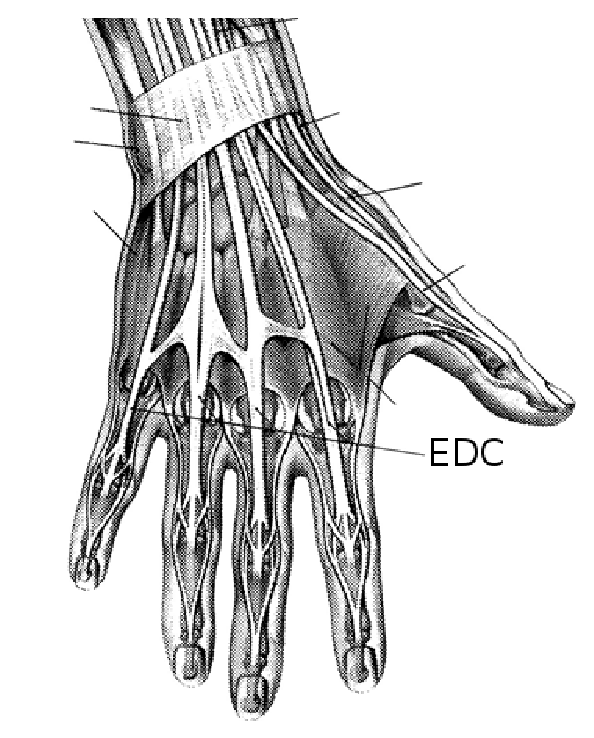
\includegraphics[width=4cm]{Handanatomy2}
\end{subfigure}
\begin{subfigure}
\includegraphics[width=4cm]{handanatomy}
\end{subfigure}
\caption{Hand Anatomy}
\label{fig:handAnatomyTotal}
\vspace{-15pt}
\end{figure}

\subsection{Deviation from Range of Rest Posture}

%rest on supports
\textbf{Range of Rest Posture (RRP)} is a range of angles for an articular joint\footnote{The word ``articular joint" refers to joints in the human body.}, where the joint ``can be considered statistically in rest"\cite{apostolico2014postural}. The resulting relaxation of muscles and tendons creates maximum comfort in this particular joint. In our case, we considered the non-resting human hand to have a specific RRP for each finger joint, when the palm is facing downwards. Combining the RRPs of each finger joint for the entire hand results in a set of relaxed hand postures where comfort is maximized.

For articular joints perceived comfort decreases when deviating from the RRP and it minimizes at the bounds of the total range of motion. Applying this to the whole hand leads to the conclusion, that hand posture comfort can be evaluated by adding up the individual joint angle distances to the RRP~\cite{naddeo2015proposal}.

In our implementation the RRP was represented by a set of 50 relaxed hand postures recorded with the Leap. The metric \textbf{RRP(x)} was simply computed by calculating the minimum euclidean distance of a hand denoted as a multi-dimensional vector ``x" to the RRP set.
For simplicity we assumed comfort to linearly decrease with distance to the RRP in our metric.

\subsection{The Inter Finger Angles}

The hand has a very compact and highly connected system of muscles and tendons that limits the individual movement of fingers (Figure \ref{fig:handAnatomyTotal}).
Aside from the thumb, fingers share \textsl{most} of their flexor and extendor muscles. Despite that minor individual flexion and extension (Figure \ref{fig:hyperabduction}) of adjacent fingers is still possible due to finger tendons originating from different areas of the muscles. In the case of the EDC (\textit{Extensor digitorum communis}) the finger tendons are even interconnected on the back of the hand (Figure \ref{fig:handAnatomyTotal}). 

Based on this, hand postures with high bending differences of adjacent fingers should lead to stress of tendons and muscles, resulting in discomfort.

The \textbf{inter finger angle component} \textbf{IFA(x)} was computed by first adding up the flexion/extension angles of MCP (\textit{metacarpophalangeal}, PIP(\textit{proximal interphalangeal}) and DIP (\textit{distal interphalangeal}) joints (Figure \ref{fig:handAnatomyTotal}) for each finger. We then added up the differences in total bending of adjacent fingers (3 values). In order to compensate anatomical differences of the fingers, mostly affecting the ring finger, we added a ring finger bonus consisting of the difference of the ring finger's bending to both of its neighbors multiplied with an estimated weight coefficient. The importance of this differentiation can be seen when the fist is closed. Extending the ring finger from a closed fist is much harder than extending the index finger. 

\begin{figure}[b]
\centering
\vspace{-10pt}
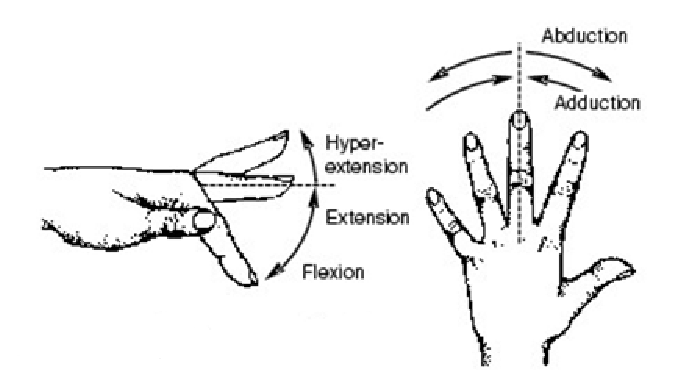
\includegraphics[width=7cm]{abduction}
\vspace{-10pt}
\caption{Hyperextension and Abduction}
\label{fig:hyperabduction}
\vspace{-10pt}
\end{figure}

\subsection{Finger Hyperextension}

\textbf{Hyperextension} (Figure \ref{fig:hyperabduction}) ``\textit{puts more strain on the }[MCP] \textit{joints and tendons than the hand is accustomed to}" and therefore causes discomfort \cite{laviola1999survey}.
Even though this might seem redundant to the deviation from RRP on first sight, hyperextension takes an increased toll as it causes considerably more discomfort, compared to a full flexion of the fingers and compared to what the deviation from RRP would suggest.

For the \textbf{hyper extension} component \textbf{HE(x)} we simply added up the flexion/extension angles of the fingers' MCPs that had a negative angle and were therefore hyperextended.

\subsection{Finger Abduction}

Finger \textbf{abduction} (Figure \ref{fig:hyperabduction})
also causes stress on the MCP joint, the abduction muscles and tendons involved.

Abduction was taken into consideration, analogue to the hyperextension, as full abduction creates substantially more discomfort than full adduction.

We computed the \textbf{abduction} component \textbf{FA(x)} by adding up the absolute abduction/adduction angle for the finger. This is possible as a fully adducted finger has an abduction angle of 0 in our model.


\subsection{Naive Metric}


Based on the model mentioned above \cite{vink2012editorial}, we then assigned the components to either comfort or discomfort. We then designed our metrics to be the added up component values \begin{math}(RRP, IFA, ...)\end{math} multiplied with weighting coefficients \begin{math}(c_{RRP(x)}, c_{IFA(x)}, ...)\end{math}. These weighting coefficients were estimated for the \textbf{naive metric.} 
	\[
	Comfort(x) = c_{RRP}\cdot RRP(x)
	\]
	\[
	Discomfort(x) = c_{IFA}\cdot IFA(x)  +  c_{HE}\cdot HE(x)  +  c_{FA}\cdot FA(x)
	\]

We hypothesize that the resulting metrics will correlate with user perception, having the value 0 as maximum  for comfort and minimum for discomfort.

\subsection{Improved Metric}

Even though the naive metrics contain the causes of comfort and discomfort, they still lack deeper consideration for the anatomical differences between the fingers.
The concept of improvement extends the thought process already used for inter finger angles: instead of applying the metrics to the whole hand, we consider the contributions from individual fingers and weight them with importance coefficients. 

	\[
	Discomfort = c_{IFAindex}\cdot IFA(index)  +  c_{IFAmiddle}\cdot...
	\]

In our case we have five comfort values and a total of twelve discomfort values. 

However, the exact weighting coefficients are generally unknown and hard to estimate. To solve this problem, we reduced it to a curve fitting problem with 17 unknowns. We used data obtained from user studies to find the correct coefficients.

\section{Methodology}

For the collection of data, we created a test environment using \textbf{Unity 3D} with a total of two tasks. In the first task, the subject would be shown a randomly generated hand posture on screen. We used our naive metric to ensure a homogenous distribution of expected comfort and discomfort. The subject was asked to mimic the hand posture with his or her dominant hand and then rate the posture. As we did not expect the subjects to be familiar with current comfort and discomfort models, we asked them to rate hand postures on an intuitive scale ranging from 0 (very uncomfortable) to 10 (very comfortable). The subject was told to rate the hand posture with 0 points if he or she was unable to reproduce it. Before beginning the evaluation, subjects were asked to form two hand postures so that they have a comfort/discomfort reference for the actual test. The first hand posture was a completely relaxed hand, the second hand posture was a randomly generated hand, that was challenging to mimic (such as the posture in figure \ref{fig:Robot}).

In the second task, the subjects were again given a randomly generated hand posture. Again the subject had to mimic the hand posture with his dominant hand and give it a rating from 0 to 10. After confirming his or her rating, the subject had to perform a target shooting task (Figure \ref{fig:participant}) with that specific posture. We tracked the subject's hand using an \textbf{ART Tracking Device}. The software showed subjects a minimalistic representation of their hand position and indicated the forward direction of their hand with a ray. Subjects were seated, with the elbow rested on a table. They had to use this ray to aim down a total of 12 targets, appearing in random order, and shoot them, by pressing a button with the off-hand. By recording the hand posture before the trial using a Leap, and checking the hand posture during the test, we made sure that the subject would not break the posture. 

\begin{figure}[h]
\centering
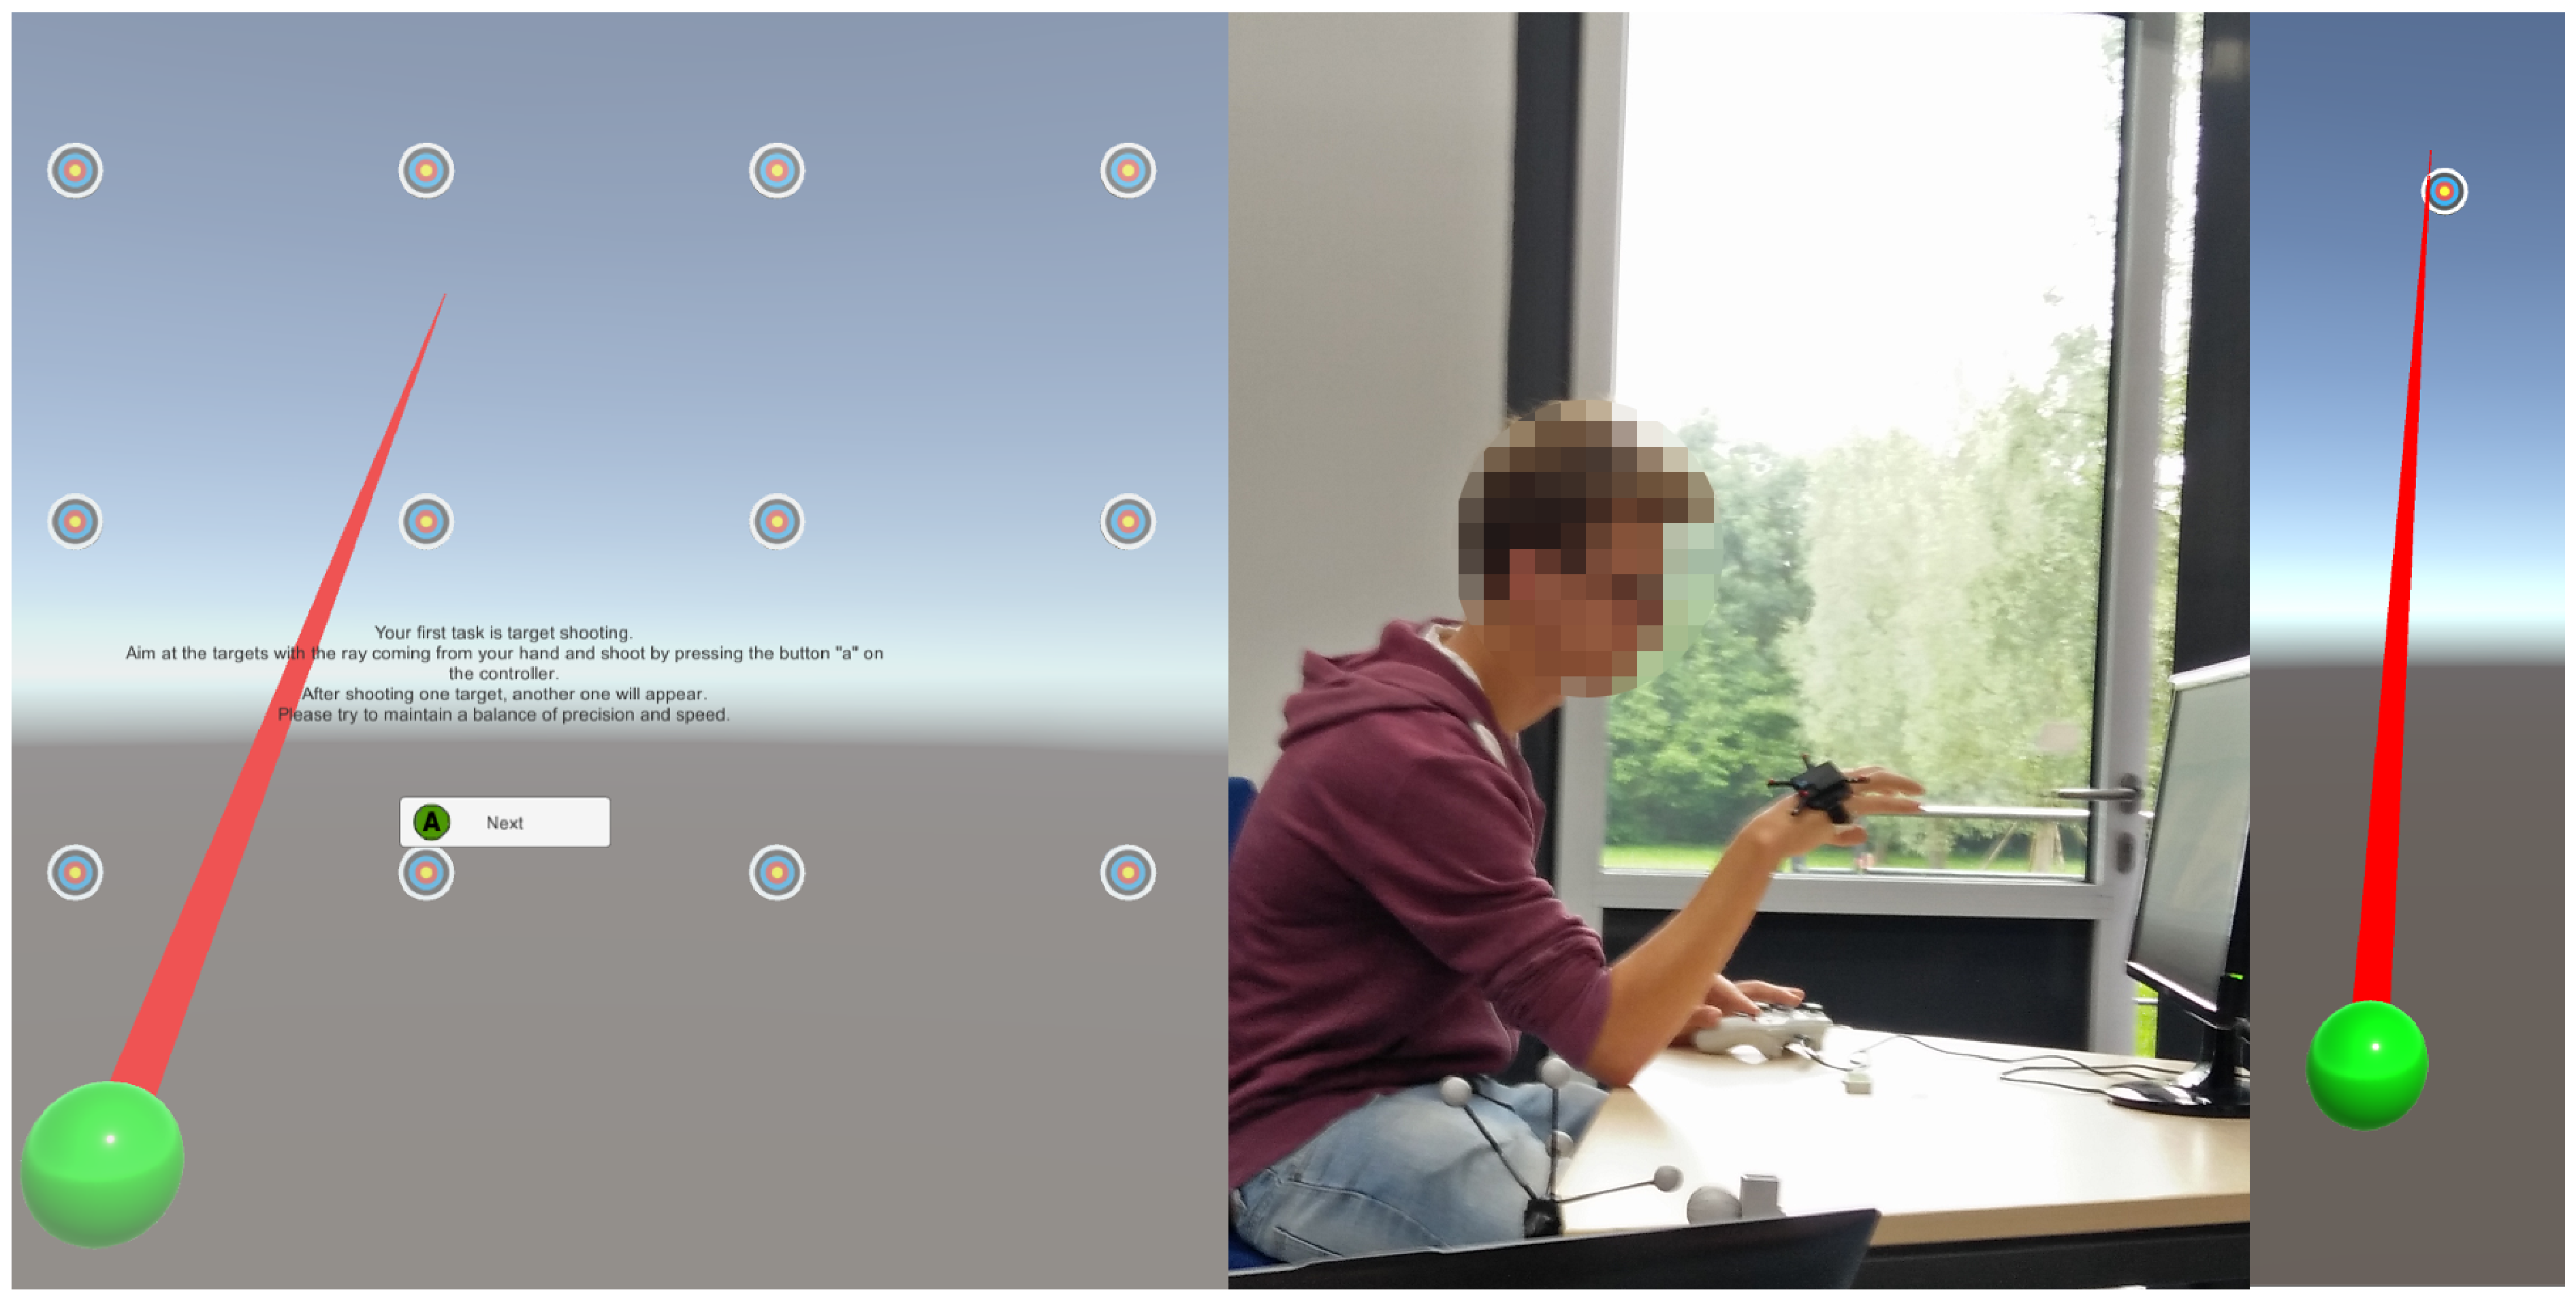
\includegraphics[width=8.45cm]{Participant}
\vspace{-20pt}
\caption{A Participant performing the Target Shooting (Best in Color)}
\label{fig:participant}
\vspace{-10pt}
\end{figure}

As a metric for performance, we measured the total time taken for the test. In order to have this affected by precision, we made the targets small and told the subjects to perform the test as quickly as possible.

We conducted a total of two user studies involving 21 participants, that resulted in 250 and 60 data sets for the metric and 35 data sets for the target shooting. Subjects were informed about the aim of the study as well as their specific objectives beforehand.

Finding the best fitting coefficients can be reduced to a curve fitting problem. Therefore we used the least squares algorithm on the first 250 data sets to fit the comfort/discomfort values to the user ratings. Afterwards we tested our results against the remaining 60 data sets to validate them. For this, we decided to combine comfort and discomfort, as we expected both comfort and discomfort to affect performance.

\section{Results \& Discussion}

\begin{figure}[b]
\centering
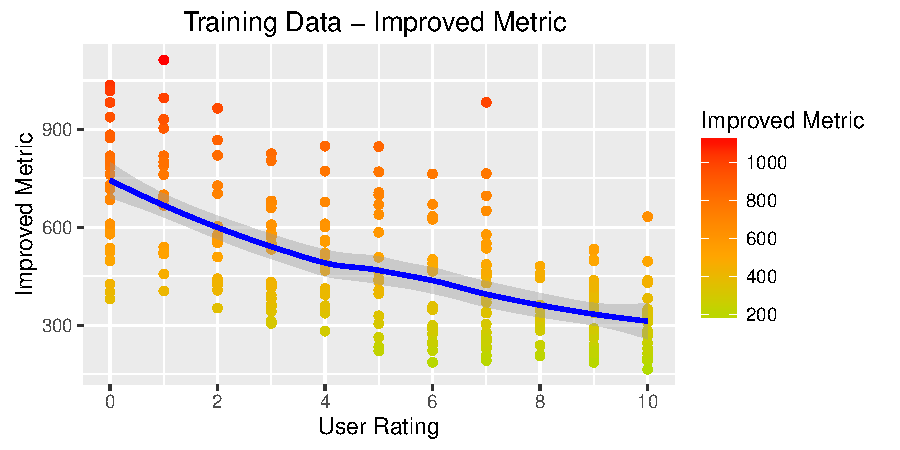
\includegraphics[width=8.45cm]{TrainingDataImproved}
\vspace{-20pt}
\caption{Improved Metric and User Rating in Training Data. \\
The Line Shows the Smoothed Conditional Mean, Calculated by the \texttt{geom\_smooth} Function in R. \\
Pearson Correlation: -0.6453242, p-value: < 2.2e-16}
\label{fig:trainingData}
\vspace{-10pt}
\end{figure}

\begin{figure}[t]
\centering
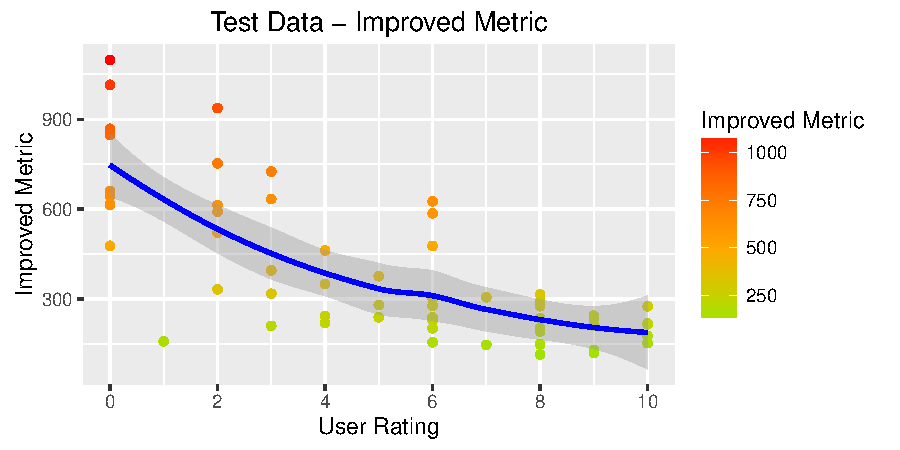
\includegraphics[width=8.45cm]{TestDataImproved}
\vspace{-20pt}
\caption{Improved Metric and User Rating in Test Data.\\
Pearson Correlation: -0.748993, p-value: 5.89e-12}
%\vspace{-5pt}
\label{fig:testData}

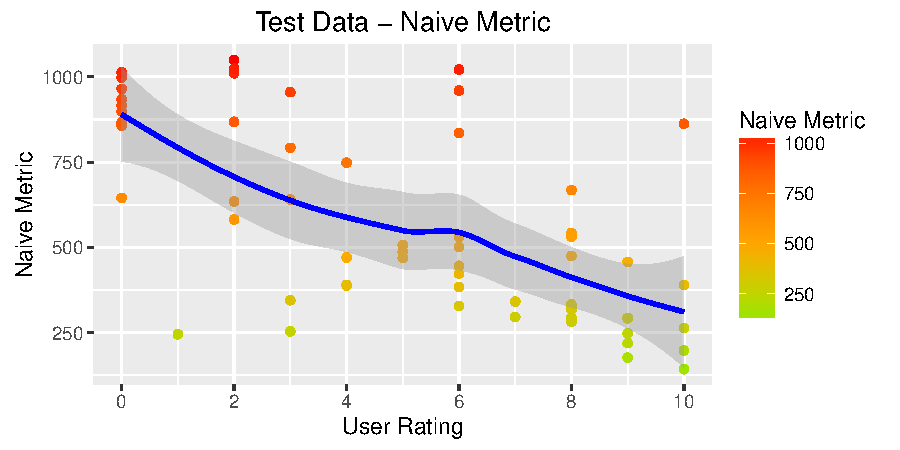
\includegraphics[width=8.45cm]{TestDataNaive}
\vspace{-20pt}
\caption{Naive Metric and User Rating in Test Data.\\
Pearson Correlation: -0.6651999, p-value: 6.73e-9}
\label{fig:testDataNaive}
\vspace{-10pt}
\end{figure}


Unsurprisingly, there was a correlation in the training data between the user rating and our improved metric, generated using this data (Figure \ref{fig:trainingData}). However, the correlation found was still not perfect, having a value of approx. \textsl{-0,65}. For this we suspect multiple reasons: 
The participants most likely had differences in anatomy and mindset, which caused them to subjectively rate comparable postures differently. In addition to that, there was little time for subjects to give their rating. Therefore long time discomfort symptoms, like pain or cramping, might not have been experienced. Finally, the subjects could only rate the hands of continuous comfort/discomfort on a scale with 11 discrete steps, which potentially introduced some additional error.

Even though the improved metric was created using a limited set of training data, it yielded a comparable correlation when applied to the test data (Figure \ref{fig:testData}). This indicates that the improved metric is a good extrapolation of the training data. Compared to the naive metric (Figure \ref{fig:testDataNaive}), there is only minor difference on first sight. However, the improved metric reduced the standard error, resulting in a better correlation and p-value.

\begin{figure}[h]
\centering
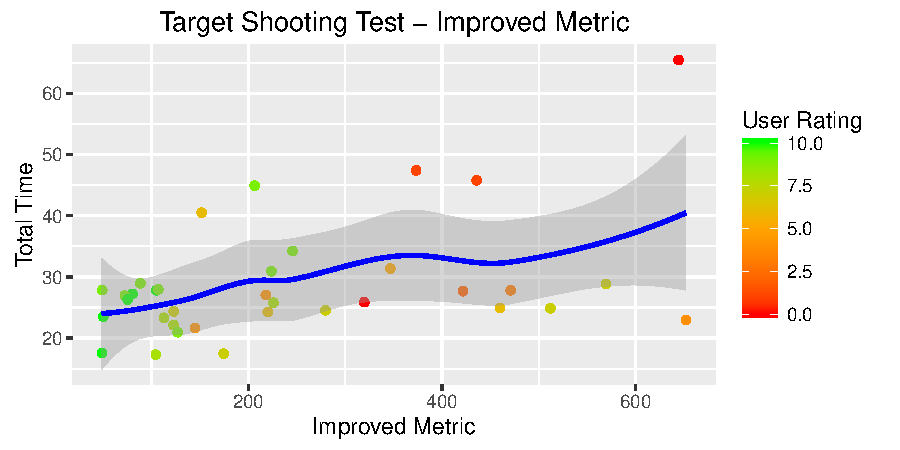
\includegraphics[width=8.45cm]{TargetShooting}
\vspace{-20pt}
\caption{Improved Metric Value and Total Task Time in Target Shooting.\\\
Pearson Correlation: -0.6651999, p-value: 6.73e-9}
\label{fig:targetShooting}
\vspace{-5pt}
\end{figure}

The results from the target shooting task (Figure \ref{fig:targetShooting}) indicate that comfort and discomfort, as measured by our metric, do affect the performance and precision in context of hand postures. This strengthens the conclusion of Short et al.~\cite{short1999precision}, that more comfortable postures generally create greater accuracy. However, the credibility of our results is limited by the relatively small number of participants. Further work is required before strong conclusions can be made.

Even though the results of this paper only apply to hand posture comfort/discomfort, the process of creating and testing a comfort/discomfort metric and its influence on performance/precision, as shown in this paper, can be transferred to other parts of the body. 

\section{Conclusion \& Future Work}
The main goal of this paper was to create a metric for quick and objective evaluation of hand posture comfort and discomfort. Furthermore we demonstrated the metric's relevance for design of hand postures, by proving its influence on precision and performance in a 3D pointing task. For the creation of the metrics we applied knowledge of hand anatomy and state of the art comfort and discomfort models and used data from a user study to improve it. Results from the testing user study suggest the improved metric to be a valid extrapolation of the training data. In addition, the outcome of a small target shooting test indicate the existence of a correlation between comfort/discomfort and precision/performance, as already suggested for different contexts in other papers.

This work neglected long term effects of a hand posture on the perceived comfort and discomfort because our envisioned usage did not assume holding the postures beyond what was necessary for issuing the command. Other contexts might need holding postures for longer and this is a potential target for future work. It would additionally be useful to determine other factors that might influence performance in a single hand task, so that we are able to design an optimum set of hand postures.

\appendix{}

\microtypesetup{protrusion=false}
\listoffigures{}
\listoftables{}
\microtypesetup{protrusion=true}
\printbibliography{}

\end{document}
